\documentclass[12pt]{article}
\usepackage{geometry}                % See geometry.pdf to learn the layout options. There are lots.
\geometry{a4paper}                   % ... or a4paper or a5paper or 
\geometry{left=2cm,right=2cm,top=2cm,bottom=2cm}
\usepackage[parfill]{parskip}    % Activate to begin paragraphs with an empty line rather than an indent

%%%%%%%%%%%%%%%%%%%%
\newcommand{\hide}[1]{}

%\usepackage[compact]{titlesec}  
%\titlespacing{\section}{0pt}{0pt}{0pt}

\usepackage{natbib}
\usepackage{xcolor}
\usepackage{url}
\usepackage{hyperref}
\usepackage{mathtools}
\usepackage{float}
\usepackage{cite}
\usepackage{tikz}
\usetikzlibrary{arrows}
\usepackage{dcolumn}
\usepackage{pdfpages}
\usepackage{booktabs}
\usepackage[verbose]{placeins}
\usepackage{blindtext}
\usepackage{tabularx}
\usepackage{array, makecell}
\usepackage{chngpage}
\usepackage{setspace}
\usepackage{placeins}
\usepackage{pifont}
\usepackage{caption}
\usepackage{subcaption}
\usepackage[numbib]{tocbibind}
\usepackage{multirow}
\usepackage{multicol}
\usepackage{color, colortbl}
\definecolor{Gray}{gray}{0.9}

\hide{
\usepackage{amscd}
\usepackage{mathptmx}
\usepackage{amsmath}
\usepackage{amssymb}
\usepackage{amsthm}
\usepackage{cases}		 
\usepackage{cutwin}
\usepackage{enumerate}
\usepackage{epstopdf}
\usepackage{graphicx}
\usepackage{ifthen}
\usepackage{lipsum}
\usepackage{mathrsfs}	
\usepackage{multimedia}
\usepackage{verbatim}
\usepackage{wrapfig}
\usepackage{appendix}
\usepackage{nameref}
}
%\bibliographystyle{chicago}

\title {Maintaining the Balance: Renewables and
European Electricity Balancing Markets}
\author{Andrew Boomer and Moongyeom Kim\\
Group 5\\
Advisor: Farid Gasmi
}

\begin{document}
\maketitle
\hspace{5cm}
\tableofcontents

\newpage
\begin{abstract}
\doublespacing
Modern economic markets are beginning to realize the scope of the inefficiency caused by the externalities related to climate change. Calls for transitioning to a carbon-free energy system to address this inefficiency are ever higher, incentivizing renewable electricity sources to capture higher shares of the market.\par

According to the theory of second best, when there are numerous inefficiencies, solving for one inefficiency does not necessarily lead to a Pareto improvement\footnote{From the paper \citet{lipsey1956general}}. While renewables may partially address the inefficiency of carbon emissions, in a complex, sub-optimal system like the electricity market, we must be cognisant of the additional inefficiencies they can introduce.\par

In this paper, we assess the impact that increasing shares of renewable electricity sources generate on maintaining grid stability. We do this by analyzing volumes in electricity balancing markets, which are currently the last resort to maintain the system's stability. We believe this paper provides value in being the first empirical econometric research into this hypothesis, where we show a robust and significant positive marginal effect, albeit small, of renewable market share on balancing volume.\par

In a broader view, we tried to show that electricity market is a complex combination of several markets and commodities where partial improvement may have unintended general equilibrium effects.

\end{abstract}

\newpage
\doublespacing
\ding{83}\ding{83} \textbf{Before reading the paper, we strongly recommend reading Appendix C: \nameref{appenidx:Background}, which would help with understanding the market and our topic of investigation.} 

\section{Introduction}
\label{section:Introduction}
\subsection{Motivation}
Shifting electricity generation resources from traditional to renewable is one of the key measures to alleviate climate change. Therefore the capacity of renewable electricity generation, especially wind and solar, has seen a rapid surge in the last two decades \citep[p. 293]{weo2018}. However, due to their weather dependence, wind and solar both show intermittent generation profiles. This variable behavior induces uncertainty in their electricity supply and can pose a strain to power grid stability. With the continuously growing share\footnote{\textbf{Figure \ref{figure:RenewEvolution}} displays the trend of VRE penetration by year, month. VRE penetration hits a maximum monthly average of over 20\% in 2019} of variable renewable electricity (VRE) in the power mix of many countries, it is important to assess their influence on balancing markets, which currently ensure power grid stability.\par

In this paper, we take an econometric approach to asses this impact, specifically by verifying whether an increase in the percentage of VRE on power grids will increase activated balancing volumes. In \textbf{Section \ref{section:Introduction}}, we introduce our hypothesis and the dataset used. In \textbf{Section \ref{section:Literature}}, we have summarized some previous literature showing the relationship between VRE penetration and procured balancing volumes in the German market. In \textbf{Section \ref{section:Model}}, we outline the development of our hypothesis as we honed in on the model that most accurately fits the characteristics and patterns of our variables. In \textbf{Section \ref{section:Result}}, we show and interpret the estimation results from our final model. \textbf{Section \ref{section:Conclusion}} concludes. \par

\subsection{Hypothesis}
We hypothesize that the increase of VRE will increase the market equilibrium quantity for activated balancing, by shifting the demand curve\footnote{It is noteworthy that the demand for balancing is perfectly inelastic, since the grid stability should be guaranteed at any cost.} to the right (\textbf{Figure \ref{figure:Hypothesis}}). The projected impact on the supply curve of activated balancing is rather ambiguous; it might shift the curve upward (Penetration of VRE could cause balancing at all volumes to be supplied by more costly generators) or downward (VRE, less-costly generators, could increase their participation at all volumes in the balancing market). The outcomes of the supply curve can be understood by analyzing how the cost of balancing changes, but we leave as an extension of the project.\par

While variables in electricity markets are often correlated with each other due to their dependence on weather and behavior, we present a simplified version outlining three possible channels of the impact of VRE on activated balancing (\textbf{Figure \ref{figure:Links}}). Though not fully comprehensive, it helps to understand why the full story can be complicated to unravel and estimate. \par

The first and most obvious channel is that the intermittent electricity generation of VRE leads to its own forecast error, thus increasing balancing needs. Second, increased VRE will affect activated balancing through various system-wide effects. For example, VRE tends to peak at certain times of the day or season, which can cause congestion in the grid system when it peaks. Additionally VRE tends to cluster in resource rich areas (think deserts for solar), and this clustering can overload local transmission systems, also causing congestion \citep{steen2014challenges}. VRE can additionally have a crowding-out effect on other resource types, which can change system flexibility in the short to medium run.\footnote{Due to their low marginal costs, VRE can temporarily alter (multi-hour or more than day long effects) the generation mix on the grid. Since electricity generators provide multi-attribute commodities (electricity, flexibility, proximity to load centers), VRE can affect adequate provision of these other attributes \citep{parsons2015financial}. This is seen in the shift of some power grids towards using quick-start gas plants to replace dwindling solar in the evening, rather than base-load resources providing electricity more evenly throughout the day. \citep{steen2014challenges}} (For characteristics of each resource, refer to \textbf{Table \ref{table:Characteristics By Sources}}) Lastly, VRE generating facilities can partially offset each other's volatility, depending on the strength and sign of correlation between generation profiles. This phenomenon could potentially lessen system-wide error, as well as enhance the stabilizing effects of integration across TSO's. For example, \citet{Ocker2017}, with a case study into the German market, found that: \begin{quote}
    "...the total demand for balancing power without a cooperation of the four TSOs in Germany would be 600MW (positive and negative). By linking the different control areas, however, the demand of balancing power drops to 300MW (only negative), since the negative and positive balancing power demands can be canceled out."\end{quote}\par

\subsection{Data}
For our analysis, we looked at the European electricity market data gathered from ENTSO-E's web-based platform dedicated to disclosure of European electricity market information (\textbf{Figure \ref{figure:Member Sates and Regional Groups}} shows all ENTSO-E member stages and Regional Groups). After data cleaning and null interpolation, we obtained a balanced panel with relatively small N (20 regions) and relatively large T (43,800: hourly data for 5 years, from the launch of the platform onward: January 2015 to the end of 2019).\par

The data is collected at different aggregation levels, due to the differing market structure across countries in the ENTSO-E footprint (i.e. Bidding Zones and Market Balance Areas, \textbf{Table \ref{table:ZoneDefinition}}). As the aggregation level of the data across variables needs to be identical, when there is a discrepancy, we merged those data collected at the smaller level to match the bigger one.\footnote{Italy, for instance, has 19 Bidding Zones and only 1 Market Balance Area. For this case, we aggregated the data collected at the bidding zone level into 1 Italian region.\\
\indent Norway, on the other hand, has 5 Market Balance Areas with each Market Balance Area corresponding one-to-one to its own Bidding Zone. We therefore were able to leave all Norwegian data as is.} Merging had to be carried out not only within country but in some cases across countries. The three-country area of Germany, Austria, and Luxembourg for example, encompasses multiple Market Balance Areas but one bidding zone (before October 2018). We therefore aggregated two Market Balance Areas to match the size of the bidding zone. Finally, we eliminated regions where the data is largely missing or inaccurate\footnote{Albania, Belarus, Bosnia and Herzegovina, Bulgaria, Croatia, Cyprus, Estonia, Finland, Greece, Iceland, Ireland, Lithuania, Latvia, Macedonia, Malta, Montenegro, Russia, Serbia, Switzerland, Turkey, the UK, and Ukraine}, reducing down to 20 regions.\par

For the remaining regions, we performed further cleaning by nullifying extreme outlying values. To fill in missing values, we carried out a stine interpolation on gaps of size one, and replaced larger gaps with the region-specific mean by hour and month. We acknowledge that this approach has its own cost of reducing the variability of the data. However, we believe this allows us to use the maximum amount of information possible from the data set.\par

It is worth mentioning, in order to further justify the data cleaning procedure we carried out, the quality and integrity of the data. Reporting compliance issues were evident in various senses; countries were not starting to provide information simultaneously at the launch of the platform, or reporting seemingly impossible numbers. We encountered many unlikely nulls and extraordinary values, which resulted in ruling out many of the regions or implementing the above null replacement procedure. \citet{Hirth2018} have analysed the platform in great depth, assessing the quality of the data and checking its external consistency (i.e. whether it coincides with other sources of the same data) and concluded: \begin{quote} "To become truly useful for industry users and researchers, both data quality and usability have to improve further."
\end{quote}

\section{Literature Review}
\label{section:Literature}
There is a wide range of scientific work on the electricity sector, covering mostly the determinants of electricity prices \citep{kyritsis2017,gil2013} and the impact of market reforms on the electricity sector \citep{erdogdu2011}. For example, \citet{hyland2016} looked at the impact of the restructuring process in the European Union on electricity prices, using a dynamic panel data regression.

However, the specific link between VRE and balancing volumes has not been studied with the same rigor. A series of studies into German balancing markets reveal that concurrently with the greater penetration of VRE into the electricity market, no greater need for balancing was found. \citet{Hirth2015a} provide an interesting statistic; though renewable energy capacity has doubled in Germany from 2008 to 2012, balancing reserves decreased by 20\% and procurement cost fell by 50\% during the same period.\par

They suggest three links to understand the impact of VRE penetration on balancing markets. First, other non-market factors such as increased Transmission System Operator (TSO) cooperation and the global recession have overcompensated for the growth of VRE. Second, with adequate market design, VRE can also act as market participants, potentially lessening their pressure on balancing markets. Lastly, the imbalance price could provide incentives for market participants to improve their forecasting accuracy.\par

\citet{Ocker2017} provide a possible explanation for the statistic found by \citet{Hirth2015a}, which is that the effect of the increased VRE share was more than offset in Germany by adaptations in the energy market design and grid control co-operations.\par

With this paper we would like to expand the realm of study into all European balancing markets, attempting to determine whether the German case can be generalized into a broader sense. Our contribution to this research topic will be to carry out a rigorous empirical analysis, which has not been attempted by the previous literature we have found.\par

\section{Model Specification}
\label{section:Model}
\subsection{Variables}
With our hypothesis, we have tried to establish the impact of VRE onto activated volumes, disentangling the most important confounding effects, as well as laying out the channels through which VRE may operate.\par

\textbf{1) Main Variables}\\
For our dependent variable, we took Activated Balancing Volume, which is the actual amount of balancing provided, as the representation of real-time strain on the grid, and not the procured balancing volume\footnote{For a detailed explanation of the balancing procurement mechanism, refer to Appendix C: \nameref{appenidx:Background}}. Our main explanatory variable is the penetration rate of VRE, given by the proportion of electricity provided by VRE generators in a given hour. \par

\textbf{2) Covariates}\\
Although in reality there could be numerous, complex, and intertwined sources that determine Activated Balancing Volume, we include only covariates that are: (a) relevant in explaining the variation in the dependent variable; and (b) correlated with the main explanatory variable of concern. These criteria are aimed towards removing omitted variable bias as well as strict relevance to our main specification of interest. The covariates included in our model are:\par

(1) VRE forecast error\\
This variable is included as per Channel 1 of our hypothesis. \textbf{Figure \ref{figure:Evolution of ActVol and RenewError}} shows the relationship between VRE forecast error and activated volumes by year and month.\par

(2) Load, Load forecast error\\
Regarding load forecast error, the deviation between the actual load and the procured day-ahead electricity for flow time can impact balancing, and hence should have explanatory power on the dependent variable. Load on its own can also influence activated balancing.\footnote{See \textbf{Figure \ref{figure:Evolution Mean of Load and ActVol}} for a comparison of the hourly shapes of Load and Activated Volumes} For example, load can exceed regional grid capacity, leading to system-wide effects such as congestion. Generally, the congestion in the Real-time Market is much greater than that of the Day-ahead Market, and therefore is often not forecast. Such real-time congestion is more likely with higher load.\\ Meanwhile, the two variables should be correlated with VRE, since both can be dependent on unpredictable weather conditions.  \par

(3) The percentage of other generation methods\footnote{Grouped in the categories such as Coal, Gas, Hydro, Nuclear and Other. These are included as percentages of the total electricity transacted in a given hour, minus those that are produced by VRE in order to distance the variables from multi-collinearity} and their forecast error\\
As the percentage of VRE generation fluctuates, the percentage of other generation methods being employed at the given hour will change, thus affecting the flexibility of the grid system. These percentages will capture part of the unobservable system-wide effects. \par
Additionally, other generation methods' forecast error can also capture volatility in production increased penetration of VRE can cause on other generation methods \citep{steen2014challenges}. 

(4) Cross-border flows\\
Cross-border flows of electricity are the result of the EU-TSO's integration. Such corss-border flow might reduce the balancing needs caused by intermittency of VRE electricity generation, as mentioned by \citet{Ocker2017}.\par

\textbf{2) Descriptive Statistics}\\
\textbf{Tables \ref{table:StatisticsOriginal}, \ref{table:StatisticsInterpolated}} show descriptive statistics of the variables included in our model, derived both from the original data and from the data after cleaning and interpolation. They are generally similar, which convinced us that analysis with the interpolated data would not skew the results in a meaningful way. Meanwhile, we have been able to see large variation in all variables in their absolute terms: Activated Balancing Volume, Percentage of VRE, Renewable Forecast Error, Imports-Exports, Load, Load Forecast Error and Other Generation's Supply Forecast Error. This is consistent with the characteristics of the electricity market, where variables exhibit significant fluctuations on an hourly basis.\par


\subsection{Initial Approach: 2SLS with Fixed Effects Model}
We determined to use Within Estimation, which eliminates time-unvarying regional heterogeneity. We chose a Fixed Effects Model over a Random Effects Model, given that the latter requires a more rigorous assumption that the individual heterogeneity is not correlated with any explanatory variables. We do not take this restrictive assumption for our specification, since the regional heterogeneity in balancing volume is likely to be correlated with explanatory variables such as load or energy mix of the region.\par

Given our initial hypothesis that more VRE does not directly cause more balancing needs, but indirectly only through increased VRE forecast error, we sought to try 2SLS estimation, with the specification laid out as below\footnote{In practice the two stages are run simultaneously in R};

\small
\textbf{First stage:}
\vspace{-0.2in}
\[\textit{VRE Forecast Error}(Z)_{i, t} = a_{i} + \alpha_{1} \textit{Renew Penetration}(X)_{i, t} +\boldsymbol{\alpha_{2}D_{t}} + \boldsymbol{\alpha_{3}F_{i, t}} + \eta_{i, t}
\vspace{-0.3in}\]
\vspace{-0.3in}
\textbf{Second stage:}
\[\textit{Activated Volume}(Y)_{i, t} = b_{i} + \beta_{1}\widehat{\textit{VRE Forecast Error}}(\hat{Z})_{i, t} + \boldsymbol{\beta_{2}D_{t}} + \boldsymbol{\beta_{3}F_{i, t}} + \varepsilon_{i, t} \]
\vspace{-0.4in}
\[where \, D_{t} = [\textit{Hour, Season, and Year dummies}],\]
\vspace{-0.5in}
\[F_{i, t} = [\textit{Load, Load Forecast Error, Cross-border Flow, Other Generation \%]}\]
\normalsize
Through preliminary correlation analysis, however, we have verified that the correlation between VRE penetration rate and VRE Forecast Error was rather weak (23\%), harming the relevance condition of the instrumental variable (\textbf{Figure \ref{figure:heatmap}}). The more important reason for abandoning the 2SLS approach, however, is the violation of the exogeneity assumption, explained in further detail below. We therefore did not run a 2SLS estimation. \par

\subsection{Further Development: Static Panel} 
We moved onto a Static Panel specification, where we included in time dummies (Yearly, Seasonally and Hourly) to correct for time fixed effects. Running the model both with and without VRE Forecast Error, we identified a statistically significant coefficient of VRE penetration rate on Activated Volumes, which contradicts our initial hypothesis of exogeneity, further confirming that VRE penetration cannot be a good instrument for VRE Forecast Error (\textbf{Table \ref{table:StaticPanel}})\par

In the meantime, we have carried out time-series analyses of the dependent variable for some sample regions, which showed trends at various levels: monthly, weekly, daily and hourly. However, such seasonality patterns were heterogeneous by countries (For full time horizon, \textbf{Figures \ref{figure:ACF1} to \ref{figure:ACF5}}; for 200 hours, \textbf{Figures \ref{figure:ACFshorter1} to \ref{figure:ACFshorter5}}), which meant that carrying out analysis without decomposition would lead to incorrect estimation of coefficients due to the violation of the parallel time-trend assumption. Consequently, we decided to discard the approach of static panel with time dummies, which do not allow us to capture such heterogeneous time effects and carry out a time series decomposition on our variables.\par

It should be mentioned, before moving onto the final model we have chosen, how we constructed our heteroscedasticity-robust standard errors. Due to the large data size, we encountered memory issues when using the sandwich package in R. To get around this, we implemented a custom function which mirrors the one utilized in R for correcting only for heteroscedasticity (not cluster-robust). The functional form for the variance-covariance matrix is 
\[(X^{'} X)^{-1} X^{'} \Sigma X (X^{'} X)^{-1} \quad \textrm{where} \quad \Sigma = diag( \hat{\epsilon} \hat{\epsilon}^{'})\]

\subsection{Final Model: Dynamic Panel}
We further hypothesized that the lagged dependent variable can capture some of the system-effects that were not fully accounted for. This provided additional reasoning for modifying our specification to a dynamic panel. Based on this result, we ultimately opted for an ARDL (Autoregressive Distributed Lag) Model, where lagged dependent variables are included as explanatory variables\footnote{We referred to the ACF graphs to determine the lags included}. These lags can partially capture spurious state dependence, as well as account for some serial correlation. Our ARDL model specification is given below. 
\vspace{-0.25in}
\begin{equation*}
    \Lambda(L)\textit{Y}_{i, t} = c_{i} + \gamma_{1}\textit{X}_{i, t} + \gamma_{2}\textit{Z}_{i, t} + \boldsymbol{\gamma_{3}F_{i, t}}
    \varepsilon_{i, t}
\end{equation*}
\[
  \textrm{ where } \Lambda(L) = (1 - \sum_{t \in T} \phi_{t} L^t)\]
\[\textbf{T} = \{1:25; \ 47:49; \ 71:73; \ 95:97; \ 119:121; \ 143:145; \ 167:169\}\footnote{These lags make intuitive economic sense given the behavior of the electricity market.}\]

We successfully tested this approach using an AR model on Activated Volumes for some sample regions (We did not reject the null hypothesis of no serial correlation with the Breush-Pagan test up to 3 to 5 lags). We ran an additional specification using the decomposed versions of the explanatory and dependent variables.

\textbf{Table \ref{table:DynamicPanel}} shows the result of the ARDL model without decomposition and \textbf{Table \ref{table:Decomposed}} show the results for Static and Dynamic models with decomposed variables. In the decomposed model without lagged dependent variables, the coefficient estimated for VRE penetration almost goes back to the level of the Static Panel. From this, we conclude that the lagged dependent variable captured some unobserved system-wide effects, and that therefore the dynamic model is a more accurate specification.  

\section{Result}
\label{section:Result}
Power grid systems are highly constrained and controlled systems, where changes to one aspect can have a nearly immediate impact on the greater system. In this sense, interpretation of our coefficients in our final decomposed ARDL panel model should be done with a holistic view. For example, a portion of the coefficient of VRE forecast error would rightly be included as a channel through which VRE can influence activated volumes, as seen in \textbf{Table \ref{table:StaticPanel}}.\footnote{Additionally, the marginal effect of coal on activated volumes is about 10 times more powerful than VRE in the opposite direction, ceterus paribus. Since VRE can have a crowding-out effect on coal generators, this could lead to an decrease in the market share of coal, increasing activated volumes via this other avenue as well.}\par
Looking at the coefficient solely on our variable of interest, VRE penetration, we see that, on average, a 1 percentage point increase in VRE penetration will lead to about a 0.1 MWh increase in activated volumes, ceterus paribus. In terms of standard deviations, a 1 standard deviation increase in VRE penetration will, on average, lead to a 0.0000057 standard deviation increase in activated volumes, ceterus paribus, a small effect to be sure. \par
Viewing our model holistically, however, the fact that all the coefficients are statistically significant would suggest that the three channels that comprise our hypothesis are all valid. At the same time, our model failed to remove persistent serial correlation in the error term (rejection of panel Breusch-Pagan test). While our time series analysis applied region-specific data, the treatment process was homogeneous across regions. Due to stark differences among our regions, a heterogeneous treatment may be necessary to fully account for the serial correlation. For the moment, we leave this extended time series analysis as a further extension of our research.

\section{Conclusion}
\label{section:Conclusion}
In order to assess the impact of the increasing penetration of VRE on grid stability, we looked at how it affects the balancing market in terms of activated volume.\par
We have been able to consistently obtain positive coefficients that are statistically significant for VRE penetration. At the same time, given that all our covariates can be considered as both controls and channels, we can argue that the fact that all the other covariates showed significant coefficients provide evidence that all our hypothesized channels of VRE's impact on Activated Volume are valid.\par
Though these findings are meaningful, considering that this is to our best understanding the first attempt to verify the impact of the VRE penetration on grid stability, for a more valid policy implication, the total cost of balancing should be studied further. It should also be considered that penetration of VRE takes place on a dynamic time horizon and that a variety of system-wide changes are simultaneously taking place, which can aggravate or alleviate any strain it causes on the grid. Increased integration of the European market and construction of transmission lines are examples of changes that can possibly offset certain negative system-wide effect that penetration of VRE can cause, as \citet{Ocker2017} found. However, these projects obviously require a thorough site-specific cost-benefit analysis.  \par
Finally, we present some possible extensions of this study. The first and most obvious one is to look into the effect on the cost of balancing. It may also be fruitful to deconstruct the panel, running individual time series models on each region, considering the heterogeneous time trends seen. Furthermore, though we have grouped wind and solar, the two have different generation profiles, and affect forecast error in unique ways. It would also be interesting to look at their individual effects on activated balancing. Lastly, we consider analyzing not just activated volumes, but the distribution of procured balancing volumes as well. In summary, the study into the balancing market is a field ripe for further research. 
\par

\newpage
\begin{appendix}

\section{Figures}
\label{appendix:Figures}

\begin{figure}[!htbp]
    \centering
      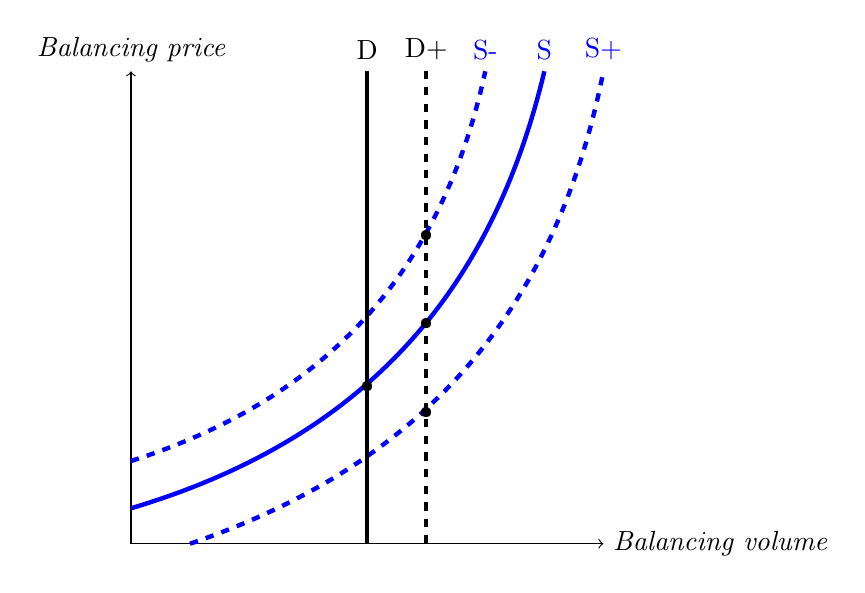
\begin{tikzpicture}[scale=3]
        \draw[->] (0,0) -- (2,0) node[right] {$\textit{Balancing volume}$}; 
        \draw[->] (0,0) -- (0,2) node[above] {$\textit{Balancing price}$};
        \draw [color = blue, ultra thick] (0, .15) to [bend right] (1.75, 2) node[above] {S};
        \draw [color = blue, dashed, ultra thick] (0, 0.35) to [bend right] (1.5, 2) node[above] {S-};
        \draw [color = blue, dashed, ultra thick] (0.25, 0) to [bend right] (2, 2) node[above] {S+};
        \draw [color = black, ultra thick] (1,0) -- (1, 2) node[above] {D};
        \draw [color = black, dashed, ultra thick] (1.25,0) -- (1.25, 2) node[above] {D+};
        \foreach \Point in {(1, 0.66), (1.25, 0.55), (1.25, 0.93), (1.25, 1.3)}
        \node at \Point {\textbullet}; 
      \end{tikzpicture}
\caption{Hypothesized reaction of the electricity market to the increase VRE penetration}
\label{figure:Hypothesis}
\end{figure}


\begin{figure}[!htbp]
\centering
    \tikzstyle{box} = [rectangle, rounded corners, minimum width=1cm, minimum height=1cm,text centered, draw=black]
    \tikzstyle{arrow} = [thick,->,>=stealth]

    \begin{tikzpicture}[node distance=2cm]
        \node (ActVol) [box, fill = green!80!black, font=\footnotesize] {\tiny Balance Volume};
        \node (EE) [box, left of = ActVol, node distance = 4cm, text width = 3.3cm, fill = red!80!black] {\tiny System-Wide Effects (Congestion, Flexibility, etc.)};
        \node (Renew) [box, left of = EE, node distance = 5cm, fill = green!80!black, font=\footnotesize] {\tiny Renew};
        \node (Weather) [box, below of = Renew, node distance = 2.8cm, fill = red!80!black, font=\footnotesize] {\tiny Weather};
        \node (RenewError) [box, above of = EE, node distance = 2cm, fill = green!80!black, font=\footnotesize] {\tiny Renew Error};
        \draw[arrow] (Weather) -- (Renew);
        \draw [arrow] (Renew) -- (RenewError) node[midway, fill = white, inner sep = 0pt] {Channel 1};
        \draw [arrow] (RenewError) -- (ActVol);
        \node (OSE) [box, below of = EE, node distance = 2cm, text width = 2.5cm, fill = green!80!black, font=\footnotesize] {\tiny Other Supply Effects (Internal + External)};
        \node (DE) [box, below of = ActVol, node distance = 2.8cm, fill = green!80!black, font=\footnotesize] {\tiny Demand Effects};
            \draw [arrow, <->] (Renew) -- (EE) node[midway, fill = white, inner sep = 0pt] {Channel 2};
            \draw [arrow] (EE) -- (ActVol);
            \draw[arrow, <->] (EE) -- (OSE);
            \draw [arrow] (OSE) -- (ActVol);
      \node (Legend) [box, above of = ActVol, node distance = 2cm, text width = 2.3cm, font=\footnotesize] {\tiny Green = Observed Red = Unobserved};
      \draw[arrow] (DE) -- (ActVol);
      \draw[arrow] (Weather) -- (DE);
      \draw[arrow] (DE) -- (EE);
      \draw[arrow, <->] (RenewError) -- (EE);
      \draw[arrow] (Renew) -- (OSE) node[midway, fill = white, inner sep = 0pt] {Channel 3};

        
    \end{tikzpicture}
    \caption{3 Channels of Effect of Increased VRE Penetration on Balance Volume}
    \label{figure:Links}
\end{figure}



\begin{figure}[!htbp]
    \begin{center}
    \includegraphics[width=10cm]{Regional_groups.png}
    \end{center}
\caption{ENTSO-e Member States and Regional Groups}
\label{figure:Member Sates and Regional Groups}
\source{\url{https://docstore.entsoe.eu/about-entso-e/system-operations/regional-groups/Pages/default.aspx}}
\end{figure}



\newpage
\begin{figure}[!htbp]
    \centering
    \includegraphics[page=1, width=\linewidth]{Graphs.pdf}
 \caption{Mean of Load and Activated Volume (Per hour for all regions)}
 \label{figure:Evolution Mean of Load and ActVol}
\end{figure}


\newpage
\begin{figure}[!htbp]
  \centering
  \includegraphics[page=3, width=\linewidth]{Graphs.pdf}
 \caption{Mean of VRE Forecast Error and Activated Volume (by month and year)}
 \label{figure:Evolution of ActVol and RenewError}
\end{figure}


\newpage
\begin{figure}[!htbp]
  \centering
  \includegraphics[page=2, width=\linewidth]{Graphs.pdf}
 \caption{Mean Penetration Rate of VRE Generation (Total, Wind, Solar by month and year)}
 \label{figure:RenewEvolution}
\end{figure}




\begin{figure}[!htbp]
    \centering
    \includegraphics[page=4, width=\textwidth]{Graphs.pdf}
    \caption{Heatmap of Correlation between Variables}
    \label{figure:heatmap}
\end{figure}




\newpage
\begin{figure}
\centering
\begin{subfigure}{.5\textwidth}
  \centering
  \includegraphics[page=6, width=\linewidth]{Graphs.pdf}
\end{subfigure}%
\begin{subfigure}{.5\textwidth}
  \centering
  \includegraphics[page=8, width=\linewidth]{Graphs.pdf}
\end{subfigure}
\begin{subfigure}{.5\textwidth}
  \centering
  \includegraphics[page=10, width=\linewidth]{Graphs.pdf}
\end{subfigure}%
\begin{subfigure}{.5\textwidth}
  \centering
  \includegraphics[page=12, width=\linewidth]{Graphs.pdf}
\end{subfigure}
\caption{ACFs of Activated Volume for Full Time Period}
\label{figure:ACF1}
\end{figure}

\newpage
\begin{figure}
\centering
\begin{subfigure}{.5\textwidth}
  \centering
  \includegraphics[page=14, width=\linewidth]{Graphs.pdf}
\end{subfigure}%
\begin{subfigure}{.5\textwidth}
  \centering
  \includegraphics[page=16, width=\linewidth]{Graphs.pdf}
\end{subfigure}
\begin{subfigure}{.5\textwidth}
  \centering
  \includegraphics[page=18, width=\linewidth]{Graphs.pdf}
\end{subfigure}%
\begin{subfigure}{.5\textwidth}
  \centering
  \includegraphics[page=20, width=\linewidth]{Graphs.pdf}
\end{subfigure}
\caption{ACFs of Activated Volume for Full Time Period}
\label{figure:ACF2}
\end{figure}

\newpage
\begin{figure}
\centering
\begin{subfigure}{.5\textwidth}
  \centering
  \includegraphics[page=22, width=\linewidth]{Graphs.pdf}
\end{subfigure}%
\begin{subfigure}{.5\textwidth}
  \centering
  \includegraphics[page=24, width=\linewidth]{Graphs.pdf}
\end{subfigure}
\begin{subfigure}{.5\textwidth}
  \centering
  \includegraphics[page=26, width=\linewidth]{Graphs.pdf}
\end{subfigure}%
\begin{subfigure}{.5\textwidth}
  \centering
  \includegraphics[page=28, width=\linewidth]{Graphs.pdf}
\end{subfigure}
\caption{ACFs of Activated Volume for Full Time Period}
\label{figure:ACF3}
\end{figure}


\newpage
\begin{figure}
\centering
\begin{subfigure}{.5\textwidth}
  \centering
  \includegraphics[page=30, width=\linewidth]{Graphs.pdf}
\end{subfigure}%
\begin{subfigure}{.5\textwidth}
  \centering
  \includegraphics[page=32, width=\linewidth]{Graphs.pdf}
\end{subfigure}
\begin{subfigure}{.5\textwidth}
  \centering
  \includegraphics[page=34, width=\linewidth]{Graphs.pdf}
\end{subfigure}%
\begin{subfigure}{.5\textwidth}
  \centering
  \includegraphics[page=36, width=\linewidth]{Graphs.pdf}
\end{subfigure}
\caption{ACFs of Activated Volume for Full Time Period}
\label{figure:ACF4}
\end{figure}


\newpage
\begin{figure}
\centering
\begin{subfigure}{.5\textwidth}
  \centering
  \includegraphics[page=38, width=\linewidth]{Graphs.pdf}
\end{subfigure}%
\begin{subfigure}{.5\textwidth}
  \centering
  \includegraphics[page=40, width=\linewidth]{Graphs.pdf}
\end{subfigure}
\begin{subfigure}{.5\textwidth}
  \centering
  \includegraphics[page=42, width=\linewidth]{Graphs.pdf}
\end{subfigure}%
\begin{subfigure}{.5\textwidth}
  \centering
  \includegraphics[page=44, width=\linewidth]{Graphs.pdf}
\end{subfigure}
\caption{ACFs of Activated Volume for Full Time Period}
\label{figure:ACF5}
\end{figure}

\newpage
\begin{figure}
\centering
\begin{subfigure}{.5\textwidth}
  \centering
  \includegraphics[page=5, width=\linewidth]{Graphs.pdf}
\end{subfigure}%
\begin{subfigure}{.5\textwidth}
  \centering
  \includegraphics[page=7, width=\linewidth]{Graphs.pdf}
\end{subfigure}
\begin{subfigure}{.5\textwidth}
  \centering
  \includegraphics[page=19, width=\linewidth]{Graphs.pdf}
\end{subfigure}%
\begin{subfigure}{.5\textwidth}
  \centering
  \includegraphics[page=11, width=\linewidth]{Graphs.pdf}
\end{subfigure}
\caption{ACFs of Activated Volume for 200 Hours}
\label{figure:ACFshorter1}
\end{figure}


\newpage
\begin{figure}
\centering
\begin{subfigure}{.5\textwidth}
  \centering
  \includegraphics[page=13, width=\linewidth]{Graphs.pdf}
\end{subfigure}%
\begin{subfigure}{.5\textwidth}
  \centering
  \includegraphics[page=15, width=\linewidth]{Graphs.pdf}
\end{subfigure}
\begin{subfigure}{.5\textwidth}
  \centering
  \includegraphics[page=17, width=\linewidth]{Graphs.pdf}
\end{subfigure}%
\begin{subfigure}{.5\textwidth}
  \centering
  \includegraphics[page=19, width=\linewidth]{Graphs.pdf}
\end{subfigure}
\caption{ACFs of Activated Volume for 200 Hours}
\label{figure:ACFshorter2}
\end{figure}


\newpage
\begin{figure}
\centering
\begin{subfigure}{.5\textwidth}
  \centering
  \includegraphics[page=21, width=\linewidth]{Graphs.pdf}
\end{subfigure}%
\begin{subfigure}{.5\textwidth}
  \centering
  \includegraphics[page=23, width=\linewidth]{Graphs.pdf}
\end{subfigure}
\begin{subfigure}{.5\textwidth}
  \centering
  \includegraphics[page=25, width=\linewidth]{Graphs.pdf}
\end{subfigure}%
\begin{subfigure}{.5\textwidth}
  \centering
  \includegraphics[page=27, width=\linewidth]{Graphs.pdf}
\end{subfigure}
\caption{ACFs of Activated Volume for 200 Hours}
\label{figure:ACFshorter3}
\end{figure}


\newpage
\begin{figure}
\centering
\begin{subfigure}{.5\textwidth}
  \centering
  \includegraphics[page=29, width=\linewidth]{Graphs.pdf}
\end{subfigure}%
\begin{subfigure}{.5\textwidth}
  \centering
  \includegraphics[page=31, width=\linewidth]{Graphs.pdf}
\end{subfigure}
\begin{subfigure}{.5\textwidth}
  \centering
  \includegraphics[page=33, width=\linewidth]{Graphs.pdf}
\end{subfigure}%
\begin{subfigure}{.5\textwidth}
  \centering
  \includegraphics[page=35, width=\linewidth]{Graphs.pdf}
\end{subfigure}
\caption{ACFs of Activated Volume for 200 Hours}
\label{figure:ACFshorter4}
\end{figure}


\newpage
\begin{figure}
\centering
\begin{subfigure}{.5\textwidth}
  \centering
  \includegraphics[page=37, width=\linewidth]{Graphs.pdf}
\end{subfigure}%
\begin{subfigure}{.5\textwidth}
  \centering
  \includegraphics[page=39, width=\linewidth]{Graphs.pdf}
\end{subfigure}
\begin{subfigure}{.5\textwidth}
  \centering
  \includegraphics[page=41, width=\linewidth]{Graphs.pdf}
\end{subfigure}%
\begin{subfigure}{.5\textwidth}
  \centering
  \includegraphics[page=43, width=\linewidth]{Graphs.pdf}
\end{subfigure}
\caption{ACFs of Activated Volume for 200 Hours}
\label{figure:ACFshorter5}
\end{figure}



\begin{figure}[!htbp]
    \centering
    \includegraphics[width=\textwidth]{"balancing reserves".jpg}
    \caption{The Four Different Balancing Reserves (Source: ENTSO-e)}
    \label{figure:reserves}
\end{figure}






\FloatBarrier

\newpage
\section{Tables}
\label{appendix:Tables}



\begin{table}[!htbp]
\centering
  \bigskip
    \small\setlength{\tabcolsep}{2pt}
        \begin{tabular}{c c c c c c}
            
           \toprule
             \textbf{Type}&\textbf{Firm/Variable}&\textbf{Type of Fuel}&\textbf{Flexibility}&\textbf{Low Carbon}&\makecell[1]{\textbf{$CO_{2}$ Emissions}\\\textbf{(kg/kWh)}} \\
           \midrule 
             \textbf{Coal} & \text{Firm} & \text{Fossil} & \text{Medium} & \text{No} & 0.95\\
             \textbf{Natural Gas} & \text{Firm} & \text{Fossil} & \text{High} & \text{No} & 0.55\\
             \textbf{Biomass} & \text{Firm} & \text{Renewable} & \text{Medium} & \multicolumn{2}{l}\text{Yes; Regrowth of biomass compensates emissions}\\
             \textbf{Nuclear} & \text{Firm} & \text{Nuclear} & \text{Low} &
             \multicolumn{2}{l}{ \multirow{5}{*}{
             \cellcolor{Gray}
             \text{Considered as zero-emission energy sources}}}\\
             \textbf{Hydro (Dam)} & \text{Firm} & \text{Renewable} & \text{Very High} &
             \multicolumn{2}{l}{
             \cellcolor{Gray}}\\
             \textbf{Solar} & \text{Variable} & \text{Renewable} & \text{Very Low}\\
             \textbf{Wind} & \text{Variable} & \text{Renewable} & \text{Very Low} &
             \multicolumn{2}{l}{
             \cellcolor{Gray}}\\
             \textbf{Geothermal} & \text{Firm} & \text{Renewable} & \text{High} &
             \multicolumn{2}{l}{
             \cellcolor{Gray}}\\
             
           \bottomrule
           \end{tabular}
\caption{Characteristics of Different Sources of Energy}
\label{table:Characteristics By Sources} 
\source{\url{https://www.europarl.europa.eu/RegData/etudes/BRIE/2016/593519/EPRS_BRI(2016)593519_EN.pdf}}
\end{table}




\begin{table}[!htbp]
\centering 
  \bigskip
    \small\setlength{\tabcolsep}{3pt}
        \begin{tabular}{l p{8cm} l p{8cm} l}
           \toprule
             \textbf{Zones} &\textbf{Description}&\textbf{Data Collected} \\
           \midrule
             \textbf{Bidding Zone} & \makecell[l]{The largest geographical area within which\\ market participants are able to bid} & \makecell[l]{\cdot \, \textit{Load}\\(Day-ahead, Actual)\\ \cdot \, \textit{Generation} \\ (Day-ahead, Actual)\\ \cdot \, \textit{Cross-border flow}} \\
            \hline 
             \makecell[1]{\textbf{Market Balance}\\ \textbf{Area}} & \makecell[l]{A geographic area for which\\an imbalance is settled at the same price} & \makecell[l]{\cdot \, \textit{Activated Balancing Volume}} \\
           \bottomrule
        \end{tabular}
\caption{Definition of various zones and data collected at each level}
\label{table:ZoneDefinition}
\end{table}


\begin{table}[!htbp] \centering
    \include{OriginalSummary}
  \caption{Descriptive Statistics: Original Data}
  \label{table:StatisticsOriginal}
\end{table}

\begin{table}[!htbp] \centering 
    \include{InterpolatedSummary}
  \caption{Descriptive Statistics: Interpolated Data}
  \label{table:StatisticsInterpolated}
\end{table}

\begin{table}[!htbp]\centering
    \include{CoefficientCompare}
    \caption{Static Panel Results}
    \label{table:StaticPanel}
\end{table}

\begin{table}[!htbp] \centering
  \include{DynamicComparison}
  \caption{Dynamic Panel Results}
  \label{table:DynamicPanel}
\end{table}

\begin{table}[!htbp] \centering 
  \include{DecomposedComparison}
  \caption{Decomposed Results}
  \label{table:Decomposed}
\end{table}


\FloatBarrier
\section{Electricity Market Background}
\label{appenidx:Background}
\caption{Appendix C: Electricity Market Background}

\subsubsection*{Load of Flow Time}\par
Flow time refers to the exact time when electrons are flowing in the system, and a chain of electricity markets exist in order to meet the load at flow time. It is important to understand this extraordinary characteristic of electricity markets: demand plays an almost entirely deterministic role in the sense that it has to be met no matter what, or risk a blackout.\\
From years in advance to minutes in advance, various types of consecutive electricity markets exist in order to correct for projection errors in the previous period and ultimately meet the flow time load. Balancing markets exist in order to provide a safety net for the projection error and extreme events.

\subsubsection*{Balancing}\par
\textbf{1) Definition of Balancing}\par
Balancing means all actions and processes through which Transmission System Operators (TSOs) continuously ensure grid stability. It can be achieved either by load or generation and also can take positive (Up regulation; generation ramp-up or negative demand response) or negative value (Down regulation; generation ramp-down or positive demand response).\par

Balancing volume is procured, or contracted in the balancing market, based on the extreme case scenario and on a minimum required amount, both of which are significantly higher than the activated volume in a normal case.\footnote{based on COMMISSION REGULATION (EU) 2017/1485
of 2 August 2017: a guideline on electricity transmission system operation}.

\textbf{2) Definition of Activated Balancing}\par
Balancing Service Providers (which, once again, can either be load- or generation-providers) bid for and commit to being called upon a day ahead, and hence the market is called the Day-ahead Balancing Market. This commitment, however, may or may not be actually realized, depending on the discrepancy of the real-time market load and the actual load at flow time.\par

Based on the promptness of balancing service provision, the balancing market is segmented into 4 markets(\ref{figure:reserves});\par

1. FCR(Frequency Containment Reserve): The reserve (load or generation) that reacts to the balancing needs within 30 seconds of interval.\\
2. aFRR (Frequency Containment Reserve with automatic activation): The reserve that reacts after 30 seconds to 15 minutes.\\
3. mFRR (Frequency Restoration Reserves with manual activation): The reserve that can fully react only after 15 minutes.\\
4. RR (Replacement Reserves): The reserve that can fully react only after 45 minutes.

\subsubsection*{Electricity Market as an Auction Market \& Merit Ordering}\par
Though there exist decentralized over-the-counter markets directly between generator and Load Serving Entities, most of the electricity needs are satisfied through centralized markets that take the form of an auction market. The markets are cleared at the quantity demanded by Load Serving Entities (based on projections) and the clearing price can be either uniform or pay-as-you-bid.\\
With differing marginal costs, different types of generators form a stepwise supply stack where variable renewable electricity (VRE), low in production cost but also low in flexbility, is located at the lower left end, and traditional energy sources such as coal, high in production cost but also high in flexibility are located at the higher right end. Under this merit-order structure, VRE generators hold an advantage over generators of traditional energy sources, which creates the possibility of a crowding-out effect.

\subsubsection*{Grid Inertia}\par
The above mentioned crowding-effect can be dangerous, since it reduces the flexibility of the grid system. A good functioning grid should contain enough inertia in order for it to cope with sudden shocks, which is mostly guaranteed by sufficient rotating mass (gas- or coal-fueled turbines or nuclear).\\
One characteristic of these stable sources of electricity is that they are slower in heating up, requiring persistent production should they be called upon in the event of extreme demand shock.\\


\section{Data Appendix}
\label{appendix:Data}
\subsection{Data collection method}
The raw data extracted from the platform is in XML files, which are then unpacked and transformed into CSV files by each generation type. We then merged the files into a single CSV file.\par

\subsection{Variables}
\subsubsection*{Activated Balancing Volume: The dependent variable}
First we took the absolute value of Activated Balancing Volume data\footnote{As explained in Appendix C. Electricity Market Background, balancing can take either positive or negative value}, since our motive is to see how much balancing is caused due to more renewable energy sources in the market, and not at which direction. Then we aggregated the data into an hourly time-frame, in order to look at the total balancing volume without causing any information-loss with too much aggregation.

\subsubsection*{VRE Penetration: The main explanatory variable}
\[\textit{VRE Penetration Rate} = \frac {\textit{Total generation by wind and solar}} {\textit{Total generation}}\]

\subsubsection*{VRE Forecast Error}
\[\textit{VRE Forecast Error} =\] \[|\textit{Day-ahead Generation Forecast for Wind and Solar}\]
\[- \textit{Actual Generation of Wind and Solar}|\]

ENTSO-E provides data on the day-ahead forecast generation amount by production methods and the actual generation. The difference would indicate the error in prediction, hence we construct the variable as forecast error. We took the absolute value to maintain consistency across variables.\par

\subsubsection*{Load}
Electricity load in the Day-ahead Market

\subsubsection*{Load Forecast Error}
\[\textit{Load Forecast Error} = |\textit{Day-ahead Load Forecast}-\textit{Actual Load}|\]

ENTSO-E provides data on the day-ahead forecast load and actual load. The difference would, in this case as well, indicate the error in prediction. Again, we took the absolute value to maintain consistency across variables.

\subsubsection*{Percentage of Other Generation Methods}
\[\textit{Percentage of Other Generation Methods} = \frac{\textit{Generation by all the other methods}} {\textit{(Total Generation - Generation by Renewable) \textsuperscript{*}}}\]

* In order to reduce down degree of mutli-collinearity, we subtract the generation of VRE from the total generation.

\subsubsection*{Other Generation Forecast Error}
\[\textit {Other Generation Forecast Error} =\] \[|\textit{Day-ahead Generation Forecast for All the Other Generation Methods}\]
\[- \textit{Actual Generation of All the Other Generation Methods}|\]

\subsubsection*{Export Import}
\[\textit{Export Import} = |\textit{Import Flow} - \textit{Export flow}| \]



\newpage
\section{Glossary}
\label{appendix:Glossary}
\textbf{Activated Balancing Volume}\\
Realized balancing, which is a portion of procured balancing\par
\textbf{Balancing}\\
All actions and processes through which TSOs continuously ensure the stability of the grid system\par
\textbf{ENTSO-E (European Network of Transmission System Operators for Electricity)}\\
Consists of 42 TSOs from 35 European countries, ENTSO-E was established and given legal mandate by the EU’s Third Legislative Package for the Internal Energy Market in 2009, which aims at further liberalising the gas and electricity markets in the EU\par
\textbf{Grid}\\
Totality of networks which connects electricity generators and consumers. Broadly divided into two parts: transmission (long-distance line) and distribution (line that connects transmission system with consumers) \par
\textbf{Grid Frequency}\\
The speed at which electrons travel in the transmission line. In the absence of balancing, a shortage of power would cause the speed to drop, risking blackouts. In an oversupply scenario, the speed would pick up, risking damage to transmission lines. Thus the speed has to be maintained at its stable level (50Hz for Europe). \par
\textbf{Load}\\
Load means the amount of electricity demanded by consumers. Load can be a forecast measure or the precise volume demanded at flow time.\\
\textbf{TSO(Transmission System Operator)}\\
Legal entity responsible for operating and maintaining, and if required, developing the transmission system in a given area\par
\textbf{VRE(Variable Renewable Energy)}\\
Refers to Wind and Solar

\newpage
\nocite{*}
\bibliographystyle{refstyle}
\bibliography{Bibliography}

\end{appendix}

\hspace{2cm}

\end{document} 
%%%%%%%%%%%%%%%%%%%%%%%%%%%%%%%%%%%%%%%%%%%%%%